\documentclass[twoside,11pt]{article}

% Any additional packages needed should be included after jmlr2e.
% Note that jmlr2e.sty includes epsfig, amssymb, natbib and graphicx,
% and defines many common macros, such as 'proof' and 'example'.
%
% It also sets the bibliographystyle to plainnat; for more information on
% natbib citation styles, see the natbib documentation, a copy of which
% is archived at http://www.jmlr.org/format/natbib.pdf

\usepackage{jmlr2e}
\usepackage{multirow}
\usepackage{booktabs}
\usepackage{xspace}
\usepackage[table]{xcolor}
\usepackage{graphicx}
\usepackage[inline]{enumitem}
\usepackage{hyperref}
\usepackage{algorithm}
\usepackage{algpseudocode}
\usepackage{amsmath,amsfonts,dsfont,mathrsfs,mathtools,amssymb}
% \newcommand{\INDSTATE}[1][1]{\STATE\hspace{#1\algorithmicindent}}
\newcommand{\INDSTATE}{\STATE\hspace{\algorithmicindent}}
\newcommand{\argmax}[1]{\underset{#1}{\operatorname{arg}\,\operatorname{max}}\;}
% \usepackage{showframe}
% \usepackage{siunitx}
% Definitions of handy macros can go here

\newcommand{\dataset}{{\cal D}}
\newcommand{\fracpartial}[2]{\frac{\partial #1}{\partial  #2}}

\newcommand{\ade}{\texttt{Adenine}\@\xspace}
\newcommand{\py}{\texttt{Python}\@\xspace}
\newcommand*{\ie}{i.e.\@\xspace}
\newcommand*{\eg}{e.g.\@\xspace}
\newcommand{\todo}[1]{\textcolor{red}{{\bf \{#1\}}}} %TODO

% Heading arguments are {volume}{year}{pages}{submitted}{published}{author-full-names}
\jmlrheading{X}{2016}{X-XX}{X/XX}{XX/XX}{Samuele Fiorini, Federico Tomasi and Annalisa Barla}

% Short headings should be running head and authors last names

\ShortHeadings{ADENINE}{Fiorini, Tomasi, Barla}
\firstpageno{1}

\begin{document}

\title{ADENINE --- A Data ExploratioN pIpeliNE}

\author{\name{Samuele Fiorini} \email{samuele.fiorini@dibris.unige.it}\\
\name{Federico Tomasi} \email{federico.tomasi@dibris.unige.it}\\
\name{Annalisa Barla} \email{annalisa.barla@unige.it}\\[1em]
\addr Department of Informatics, Bioengineering, \\Robotics and System Engineering (DIBRIS)\\
     University of Genoa\\
     Genoa, I-16146, Italy}


\editor{Editor name}

\maketitle

\begin{abstract}

In this paper we introduce \ade, a machine learning \py framework for data exploration. The main goals of \ade, is twofold: helping researchers and data scientists achieving a first and quick overview on the main structures underlying their data and choosing the most suitable unsupervised learning pipeline for the problem at hand. This software tool encompasses state of the art techniques for: missing values imputing, preprocessing, dimensionality reduction and clustering tasks.
\ade exploits both process and thread level parallelism and it is capable of generating nice and clean publication-ready figures along with quantitative descriptions of the pipelines performance. \ade is released under FreeBSD license and it can be downloaded from \href{http://slipguru.github.io/adenine/}{http://slipguru.github.io/adenine/}.
%% max 200 words: current ~100

\end{abstract}

\begin{keywords}
Data exploration, unsupervised learning, RNA-Seq gene expression
\end{keywords}

\section{Introduction}\label{sec:intro}
Data exploration is a very insightful starting point for many data analysis projects. Researchers and data scientists are often asked to extract meaningful information from collections of complex and possibly high-dimensional data coming from heterogenous contexts. For instance, in biomedical scenarios, physicians are likely to be interested in answering some biological questions starting from a set of observations collected from a pool of subjects enrolled in a study. Possible investigations can be: \emph{is there any relevant stratification among subjects?} or \emph{is it possible to discriminate between cases and controls from my observations?}. Starting from a given dataset, the information needed to answer such questions may be immediate, non-trivial to extract or even completely absent.
In these situations, a preliminary data exploration step is not only good practice, but also a fundamental starting point for further and deeper investigations. In this context, several machine learning and data mining techniques were developed over the years. Among those we focus on the four most popular classes of methods: \begin{enumerate*}[label=(\roman*)]
  \item missing values imputing,
  \item data preprocessing,
  \item dimensionality reduction and
  \item unsupervised clustering
\end{enumerate*}.

In the last few years, a fair number of data exploration softwares and libraries  were released. At a very coarse grain we can group them into two sets: interactive GUI-based and non-interactive script-based  applications. Of the first group, we recall \emph{Divvy} \citep{lewis2013divvy}, a software tool that performs dimensionality reduction and clustering on input datasets. \emph{Divvy} is a light framework, although its interface is designed to be Mac OS X specific, it heavily lacks in documentation, its collection of \texttt{C/C++} algorithm implementations does not cover common strategies such as kernel principal component analysis (KPCA) \citep{scholkopf1997kernel} or hierarchical clustering \citep{friedman2001elements} and it does not offer strategies to perform automatic discoveries of the number of clusters. The most notable project that spans between the two families is \emph{Orange} \citep{demvsar2013orange}, a data mining software suite that offers both visual programming front-end and standard \py APIs. In the context of data exploration, \emph{Orange} can be successfully employed. However, it does not support automatic pipeline generation, hence it requires the user to manually create each pipeline. On the other hand, as of today \emph{Orange} lacks in several nonlinear methods such as spectral embedding \citep{ng2002spectral}, locally linear embedding \citep{roweis2000nonlinear} and spectral vlustering \citep{shi2000normalized}.

We introduce \ade, a script-based \py tool for data exploration that, starting from a set of predefined unsupervised algorithms, creates textual an graphical reports of an arbitrary number of pipelines. In this context data imputing, preprocessing, dimenionality reduction and clustering strategies are considered as pipeline building blocks. The user is only required to specify input data and to select blocks, then \ade takes care of automatically generate and run the pipelines made by all possible combinations of the selected algorithms. Every algorithm implementation of \ade is inherited, or extended, from \texttt{scikit-learn} \citep{scikit-learn} which is, to the best of our knowledge, the most complete machine learning open source library freely available online.

%%%%%%%%%%%%%%%%%%%%%%%%%%%%%%%%%%%%%%%%%%%%%%%%%%%%%%%%%%%%%%%%%%%%%%%%

\section{Tool overview}\label{sec:implem}
\ade is developed around the concept of \emph{pipeline}, with that we mean a sequence of the following four fundamental steps:
\begin{enumerate*}[label=(\roman*)]
  \item missing values imputing,
  \item data preprocessing,
  \item dimensionality reduction and
  \item unsupervised clustering
\end{enumerate*} (see Figure~\ref{fig:workflow}).
For each task, a fair number of off-the-shelf algorithms are available (see Table~\ref{sec:implem}), although none of these steps are mandatory and they can be skipped if not needed.

\begin{figure}[h!]
    \centering
    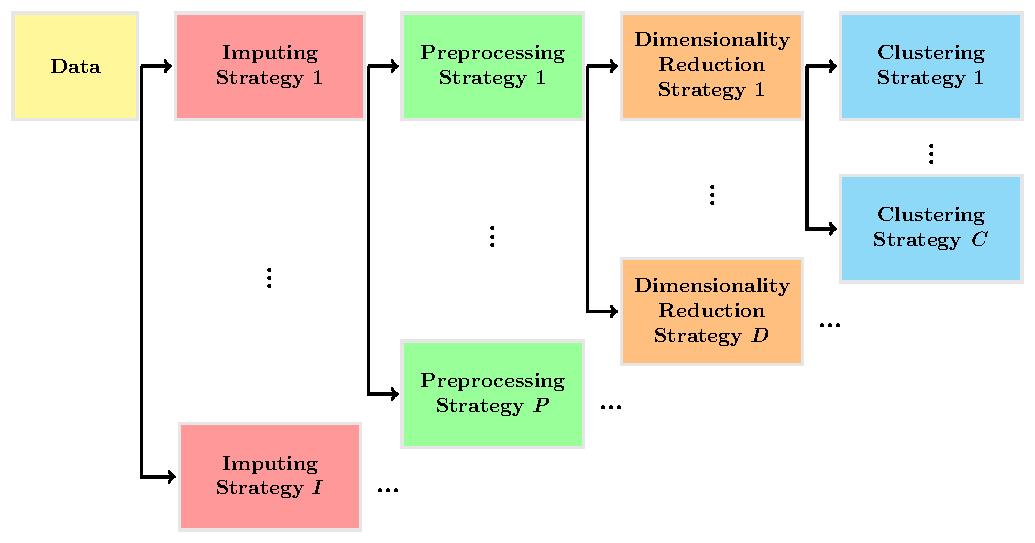
\includegraphics[width=\textwidth]{ade_wf/ade_wf.pdf}
    \caption{A schematic representation of the \ade workflow. The list of building blocks available for each step is summarized in Table~\ref{tab:blocks}. The final number of pipelines generated is $I \times P \times D \times C$.}\label{fig:workflow}
\end{figure}

\begin{enumerate}
  \item[]{\bf Step 0: Missing values imputing.}
  % \subsection*{Missing values imputing}
  Working with real-world collections of data it often happens that sets of entries are missing. In order to cope with this issue, \ade offers an improved version of the \texttt{Imputer} class offered by \texttt{scikit-learn}. Our extension adds a k-nearest neighbor (KNN) imputing method to the pre-existent features-wise \emph{mean}, \emph{median} and \emph{most frequent} value strategies.
  % (whose names are already self-explanatory)
  We chose to add the KNN imputing method to the \emph{na\"ive} strategies offered by \texttt{scikit-learn} because of its simplicity and the robustness demonstrated in the microarray reconstruction experiments described in \citep{troyanskaya2001missing}.

  \item[]{\bf Step 1: Data preprocessing.}
  % \subsection*{Data preprocessing}
  Collecting data from heterogenous sources may imply dealing with features lying in very different numerical ranges. This can sometimes have a negative influence on the behaviour of dimensionality reduction and clustering techniques. To tackle this issue \ade offers four different strategies:
  \begin{enumerate}[label=(\roman*)]
    \item \emph{Recenter}: transforming samples in order to have zero-mean;
    \item \emph{Standardize}: transforming recentered samples in order to have unit-variance;
    \item \emph{Normalize}: scaling samples in order to have $\ell^p$ unitary norm (with $p = 1$ or $2$);
    \item \emph{MinMax}: scaling features to a given range, this transformation can be expressed as
    \[
      X_{MinMax} = \frac{X - min(X)}{max(X) - min(X)} \cdot \Big[max(X) - min(X)\Big] + min(X)
    \]
    where $min$ and $max$ denote, respectively, feature-wise minimum and maximum values operators.
  \end{enumerate}

  \item[]{\bf Step 2: Dimensionality reduction.}
  % \subsection*{Dimensionality reduction}
  Data exploration of high dimensional dataset can be very tricky. Visualizing samples in high dimension is much less intuitive than representing them in basic two or three-dimensional scatterplots. Moreover, it is often possible to \emph{decrease} the dimensionality of the problem estimating, by means of different strategies, a low-dimensional embedding in which the data lie. To accomplish this task, \ade offers a set of linear and nonlinear dimensionality reduction and manifold learning algorithms, see Table~\ref{tab:blocks} for the full list of available strategies and the correspondent references.

  \item[]{\bf Step 3: Unsupervised clustering.}
  % \subsection*{Unsupervised clustering}
  Cluster analysis, when needed, are the last step of each pipeline. \ade offers different strategies ad heuristics to automatically estimate the most suitable number of clusters in a given dataset. The available clustering techniques can be grouped into centroid-based and not centroid-based methods. For the first class of methods, the optimal parameter choice follows the $B$-fold cross-validation strategy presented in Algorithm~\ref{alg:clusters}, where $\mathcal{S}(X,y)$ is defined as the mean silhouette coefficient \citep{rousseeuw1987silhouettes} for all input samples.
  The tuning parameter for the affinity propagation technique \citep{frey2007clustering} is the so-called \emph{preference} and it defines the number of discovered clusters $k$. For k-means \citep{bishop2006pattern} the tuning parameter is directly the \emph{number of clusters}, while the mean shift strategy \citep{comaniciu2002mean} has an implicit clusters discovery. For hierarchical \citep{friedman2001elements} and spectral clustering \citep{shi2000normalized} no automatic number of clusters discovery is offered. However graphical aids to evaluate the performance with fixed $k$ are generated as, respectively, dendrogram tree and plot of the eigenvalues of the Laplacian of the affinity matrix.

  \begin{algorithm}[h!]
      \caption{Automatic discovery of the optimal clustering parameter.}\label{alg:clusters}
        \begin{algorithmic}[1]
            \For{clustering parameter $k$ in $k_1 \dots k_K$ }
              \For{cross-validation split $b$ in $1 \dots B$}{\\
                \INDSTATE \INDSTATE $X^{tr}_b,X^{vld}_b\leftarrow$ $b$-th training, validation set\\
                \INDSTATE \INDSTATE $\hat{m}\leftarrow$ fit model on $X^{tr}_b$ \\
                \INDSTATE \INDSTATE $\hat{y}\leftarrow$ predict labels of $X^{vld}_b$ according to $\hat{m}$\\
                \INDSTATE \INDSTATE $s_b\leftarrow$ evaluate silhouette score  $\mathcal{S}(X^{vld}_b,\hat{y})$
                }
              \EndFor \\
              \INDSTATE $\bar{S}_k = \frac{1}{B}\sum_{i=1}^B s_i$
            \EndFor \\
            $k_{opt} = \argmax{k}(\bar{S}_k)$
          \end{algorithmic}
  \end{algorithm}

\end{enumerate}

\noindent In order to perform exploratory analysis of large datasets, \ade takes advantage of different parallel computing paradigms. For instance, its pipelines are designed to be independent from each other, therefore they all run in parallel as separate \py processes on different cores. Moreover, since \ade makes large use of \texttt{numpy} and \texttt{scipy}, it automatically benefits from their bindings with optimized linear algebra libraries (such as OpenBLAS\footnote{\href{http://www.openblas.net/}{http://www.openblas.net/}}, or Intel\textsuperscript{\textregistered}~MKL).

\section{Usage Example}
Comparing pipelines performance on toy dataset.


\section{Experiments and results}
To assess the quality of the obtained results, we tested \ade on a set of synthetic and real dataset.

\todo{parla qui dei test synth}
\todo{TGCA}

% \section{Conclusions}

%%%%%%%%%%%%%%%%%%%%%%%%%%%%%%%%%%%%%%%%%%%%%%%%%%%%%%%%%%%%%%%%%%%%%%%%%%%%%%%%%%%

\begin{table}[hbtp]
  {\caption{Pipelines building blocks and their references (not specified when the definition is given in Section~\ref{sec:implem}).}\label{tab:blocks}}

  {\begin{tabular}{lll}
  \toprule
  \bfseries Step &   \bfseries Algorithms & \bfseries Ref.\\

  \multirow{2}{*}{Imputing} & mean &  \\
  & median & \\
  & most frequent & \\
  & KNN & \citep{troyanskaya2001missing} \\
  \midrule

  \multirow{4}{*}{Preprocessing} & recentering &  \\
  & standardize &  \\
  & normalize &  \\
  & min-max &  \\
  \midrule

  \multirow{9}{*}{\begin{tabular}{@{}c@{}}Dimensionality \\ reduction\end{tabular}} & PCA & \citep{jolliffe2002principal} \\
  & incremental PCA & \citep{ross2008incremental} \\
  & randomized PCA & \citep{halko2011finding} \\
  & kernel PCA & \citep{scholkopf1997kernel} \\
  & isomap & \citep{tenenbaum2000global} \\
  & locally linear embedding & \citep{roweis2000nonlinear} \\
  & spectral embedding & \citep{ng2002spectral} \\
  & multidimensional scaling & \citep{borg2005modern} \\
  & \begin{tabular}{@{}l@{}}t-distributed stochastic \\ neighbor embedding (t-SNE)\end{tabular}   & \citep{van2008visualizing} \\
  \midrule

  \multirow{5}{*}{Clustering} & k-means &  \citep{bishop2006pattern}\\
  & affinity propagation & \citep{frey2007clustering} \\
  & mean shift & \citep{comaniciu2002mean} \\
  & spectral & \citep{shi2000normalized} \\
  & hierarchical & \citep{friedman2001elements} \\

  \bottomrule
  \end{tabular}}
\end{table}

% \acks{Acknowledgements go here.}

\vskip 0.2in
\bibliography{adenine}

\end{document}
